\documentclass{report}
\usepackage{graphicx} % Required for inserting images
%\usepackage{minted}
\usepackage[outputdir=../../]{minted} % for Overleaf compatibility
\usepackage{multirow}
\usepackage{a4wide}
\usepackage{fancyhdr}
\usepackage{amsfonts}
\usepackage{amsmath}
\usepackage{subcaption}
\usepackage{tcolorbox}
\usepackage{color}
\pagestyle{fancy}
\newcommand{\docTitle}{Multi bunch feedback application software}
\newcommand\abs[1]{\left|#1\right|}
\rhead{\docTitle}
\lhead{}
\usepackage{hyperref}
\hypersetup{
    colorlinks=true,
    linkcolor=blue,
    filecolor=magenta,      
    urlcolor=blue,
    pdftitle={Overleaf Example},
    pdfpagemode=FullScreen,
    }

\begin{document}
\title{\docTitle}
\author{Alun Morgan}
\date{June 2024}

\maketitle

\tableofcontents
\clearpage
\chapter{Conceptual descriptions}
\section{Overview}
The hardware for multi bunch feedback has many different possible configurations. Broadly speaking a feedback system has a frontend which takes in the signals from the pickups, and does the initial analogue signal conditioning. These signals are then fed into digital systems for each of the three planes (x,y,s). These digital systems calculate the feedback required and send signals to analogue drive electronics in order to excite the beam in the given plane. This is summarised in figure \ref{system_overview}

\begin{figure}[hbt]
\begin{center}
  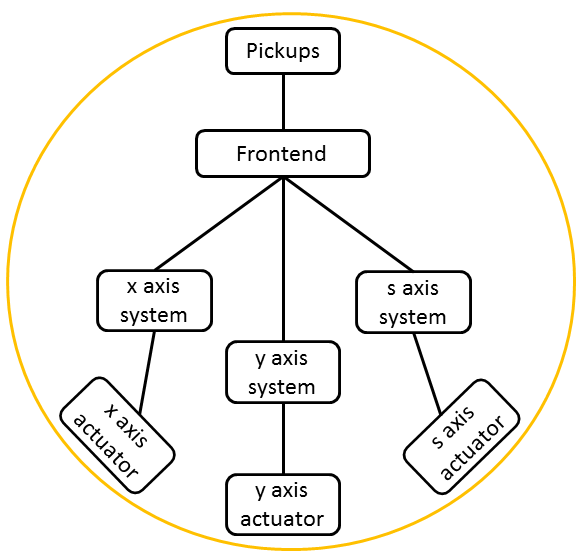
\includegraphics[width=0.5\textwidth]{top_level_system_overview.png}\\
  \caption{System overview}\label{system_overview}
\end{center}
\end{figure}

In order to make such a system more easily usable for a wide range of system users, this suite of task specific applications has been developed. The aim of the suite is to abstract away the implementation detail of the hardware and thus allow the users to put their attention on type of measurement they want to do. This abstraction also aids in the development of bespoke measurements for specific investigations.

All these codes save the relevant data and graphs to a file structure based on the date, and given unique names based on the date and time the application was run. The root path for this structure is defined in \verb|mbf_system_config.m|, as is the harmonic number of the machine under study. In general all machine/deployment parameters are set in this file. The rest of the codebase it written to adapt to what is set here.

In addition to the system data from the multi bunch hardware, more general machine parameters are also captured for growdamp, modescan and bunch motion codes, in order to enable machine studies (e.g current dependence). This additional data is set in \verb|machine_environment.m|.

\subsection{Frontend Optimisation}
In order to work optimally the feedback systems need to be matched in timing/phase with the beam phase (not the RF phase) and be tuned so that the sampling point of the ADC coincides with the maximum signal from each bunch.

The first requirement is done by phase shifting the input signal. At its most basic this comprises of a single phase shifter for each channel which both allows each channel to be adjusted to follow changes in beam phase, and to allow the axis to be  tuned in order to account for differences in the phase delay of that channel.

The practical implementation will depend on the details of your frontend hardware.
However is often realised as a single LO phase shifter which is common to all axes and handles the beam phase adjustments. meanwhile each channel has an individual additional phase shifter to tune out the systemic differences in phase delay between the channels. Such a setup is shown in figure \ref{fig:phase_shifters}.
Another variation is replacing the LO phase shifter with an automatic beam phase following system such as a DORIS ((Delayed Orbit Reference Improvement Scheme) unit which locks the MBF to a fixed relationship to beam phase rather than the RF phase. 
DORIS will lock if there is more than 3~mA in the storage ring.

The second requirement is done by adjusting the sampling clock until a maximum signal is obtained with a minimum signal leakage to adjacent RF buckets. See figure \ref{fig:frontend_clock_phase_scan} for an example.
\begin{figure}[hbt]
    \centering
        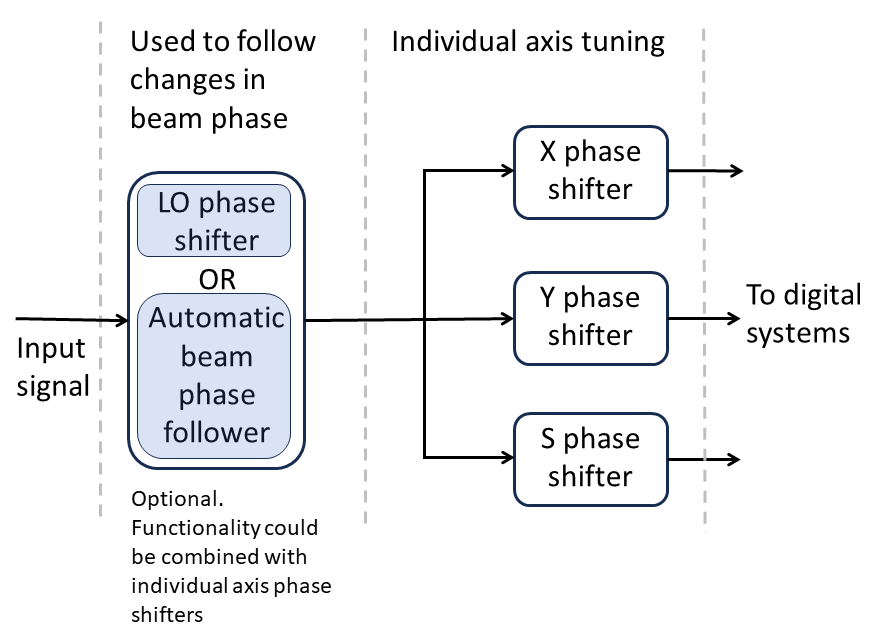
\includegraphics[width=0.9\textwidth]{phase_shifters_overview.png}
        \caption{phase shifters}
        \label{fig:phase_shifters}
\end{figure}


Note: The Libera bunch by bunch frontend seems to get into problems when scanning the LO phase shifter. It is probably best not to scan the LO phase if you have that frontend.
\clearpage
\subsection{Measurements}
\subsubsection{Frontend scans}
Scan the relevant phase shifter or clock delay while monitoring the measure signal amplitude. The resulting graphs will allow appropriate working points to be set.

\subsubsection{Mode scans}
A mode scan is a sequential excitation of the harmonics of the tune frequency. This is mainly a system check in order to identify any performance limitations or degradation.

\subsubsection{Spectra}
This code captures the requested number of turns from the requested axis and returns the FFT of the centroid motion of each bunch. This is useful for identifying tunes, tune leakage from one axis to another, also for classifying instabilities.

\subsubsection{Growdamp}
The measurement comprises a series of excitations at set harmonics of the tune frequency followed by capture of the evolution of bunch centroid positions, both with and without feedback active.

\subsubsection{Transverse damping}

\subsubsection{Emittance control}
This uses one of the oscillators to excite the selected bunches at one of the sideband frequencies. This has the effect of blowing up the beam.

\subsubsection{Bunch motion capture}
The three systems are setup to be ready to capture on the next external trigger. Once that trigger arrives, the three systems simultaneously capture bunch centroid motion. This is useful for capturing injection transients. 

\chapter{Practical use}
\section{Code location }
The code is released under an MIT licence. In order to use it please grab it from the \href{https://github.com/alunmorgan/Multi-bunch-feedback-applications}{code repository}
or use the following command on the system command line in order to copy it to your current location:
\begin{verbatim}
git clone https://github.com/alunmorgan/Multi-bunch-feedback-applications.git
\end{verbatim}
and add the resulting folder to your Matlab path. If you find odd behaviour check that you do not have any other code in the Matlab path as you could have name clashes.

If you have already cloned the repository navigate to the folder and run 
\begin{verbatim}
git pull
\end{verbatim}
This will ensure you have the most up to date version of the code.

This and related documentation can be found in the \href{https://github.com/alunmorgan/Multi-bunch-feedback-applications/Documentation}{documentation folder in the repository}

\section{MBF frontend open loop setup}
 Insertion devices (IDs) need to be set to injection gaps.
\subsection{DORIS phase}
\subsubsection{Machine settings}
Inject a full fill 10~mA.
\subsubsection{DORIS phase scan}
Before running the code to scan the DORIS phase, select a single bunch to look at.
Make sure the single bunch location has charge in it.
\begin{minted}{matlab}
    >> single_bunch_location = 400 % for example. This will select a single bunch in bucket 400.
\end{minted}
The following code will scan the phase of the DORIS unit to identify an optimum value.
\begin{minted}{matlab}
    >> DORIS_target_phase_scan(single_bunch_location) 
\end{minted}
If you want to check that the settings are changing as expected then look at the screen in figure \ref{fig:DORIS_settings} (Diagnostics $\rightarrow$ {\color{red}????}).
\begin{figure}
    \centering
    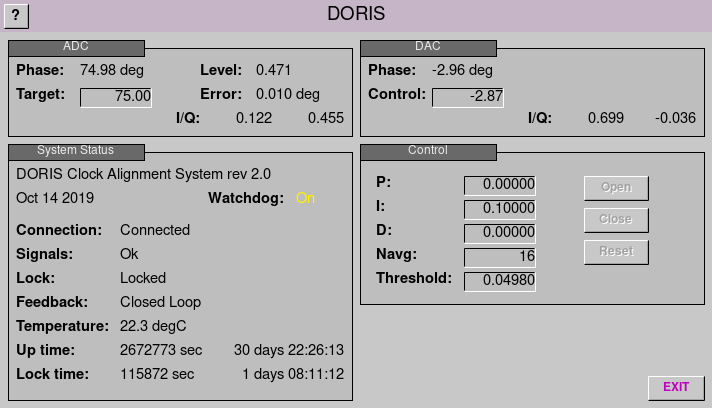
\includegraphics[width=0.8\linewidth]{DORIS_settings.png}
    \caption{DORIS settings}
    \label{fig:DORIS_settings}
\end{figure}

Figure \ref{fig:DORIS_phase_scan} shows an example of the output.
\begin{figure}[ht]
    \centering
    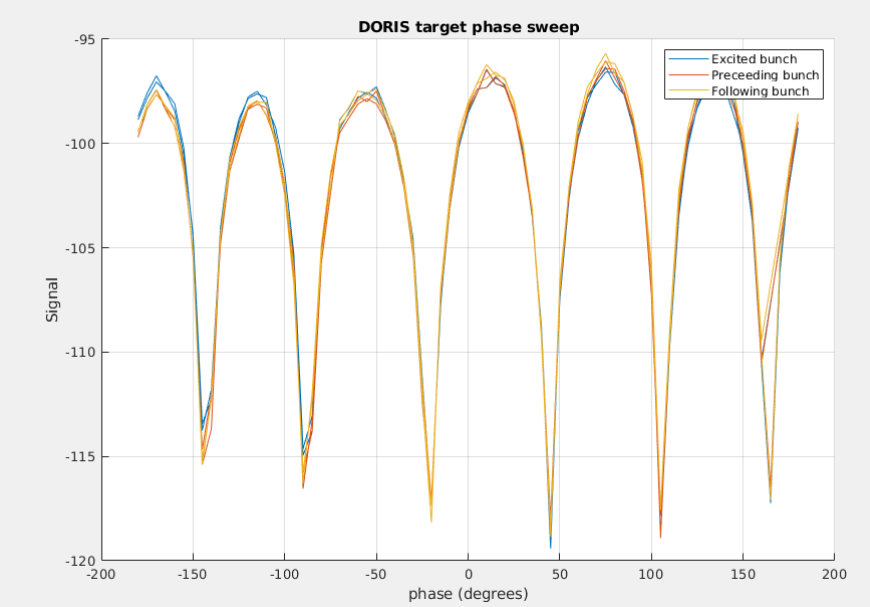
\includegraphics[width=0.8\linewidth]{DORIS_scan.png}
    \caption{In this case $75^\circ$ looks to be a reasonable working point.}
    \label{fig:DORIS_phase_scan}
\end{figure}

The optimum value is the phase where one gets the maximum signal of the excited bunch. Adjust the DORIS target phase to this phase value.
\clearpage


\subsection{Frontend phases} 
In the front end there are two phases (delays) we are interested in optimising. The system phase which determines how accurately our detectors are aligned with the target bunch, and the clock phase which determines how close to the peak of the signal we are sampling. 
\subsubsection{Machine settings}
\begin{itemize}
    \item {Inject a single bunch into a selected RF bucket (~0.2nC).}
     \item{if no sync press sync button as shown on figure \ref{fig:MBF_delays} (Diagnostics $\rightarrow$ {\color{red}????})}
    \item{Compare the MBF ADC data and the fillpattern to the bunch number requested.}
    \begin{itemize}
        \item{Look at the Bunch motion standard deviation. - \color{red}{ADD SCREENSHOT}}
        \item{Look at fill pattern (Diagnostics $\rightarrow$ Photon counting system $\rightarrow$ fill) - \color{red}{ADD SCREENSHOT}}
    \end{itemize}
    \item{adjust MBF and fillpattern until they agree with the requested bunch number as given by the timing system.}
    \begin{itemize}
    \item{adjust MBF bunch value as shown on figure \ref{fig:MBF_delays}}
    \begin{figure}[h]
        \centering
        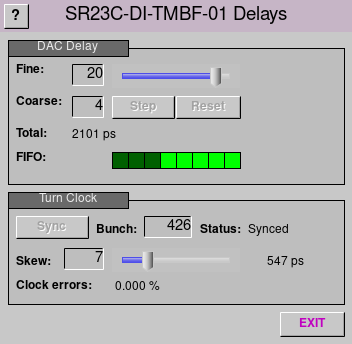
\includegraphics[width=0.6\linewidth]{MBF_delays.png}
        \caption{MBF delay screen}
        \label{fig:MBF_delays}
    \end{figure}
       
    \end{itemize}
\end{itemize}
\begin{figure}
    \centering
    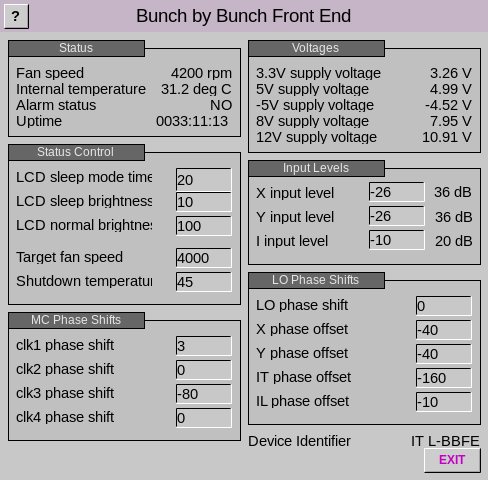
\includegraphics[width=0.6\linewidth]{BBBFE_settings.png}
    \caption{Frontend settings: System phases in LO Phase shifts section  X=X, Y=Y S=IT. Clock phases in the MC Phase Shifts section X and Y=clk3, S=clk4}
    \label{fig:BBBFE_settings}
\end{figure}
\clearpage


\subsubsection{System phase scan}
 
The following Matlab code will run a system phase scan on each axis sequentially. The graphs will be displayed, and the data is automatically stored. 

\begin{minted}{matlab}
    >> BBBFE_system_phase_scan('X', single_bunch_location)
    >> BBBFE_system_phase_scan('Y', single_bunch_location)
    >> BBBFE_system_phase_scan('S', single_bunch_location)
\end{minted}

Figure \ref{fig:frontend_system_phase_scan} shows an example of the output. You are looking for the phase value with the largest gap between the excited bunch and each of the other bunches. But also fairly near the maximum excited bunch maximum amplitude.

\begin{figure}[hbt]
   \centering
    \begin{subfigure}[b]{0.45\textwidth}
        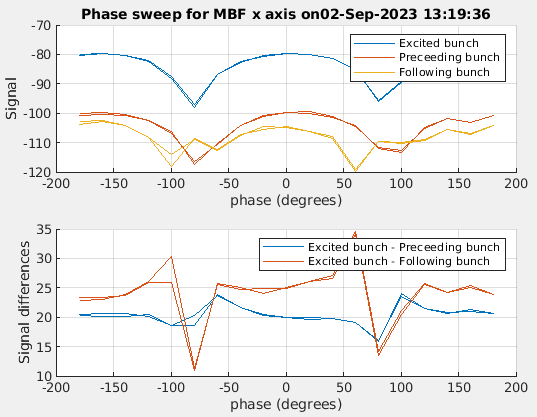
\includegraphics[width=\textwidth]{vlr_system_phase_scan_x.png}
        \caption{Horizontal axis: Anywhere between $-60^\circ$ and $0^\circ$ looks to be a reasonable working point as you are trading of better selectivity for better signal to noise.}
        \label{fig:frontend_system_phase_scan_x}
    \end{subfigure}
    \begin{subfigure}[b]{0.45\textwidth}
        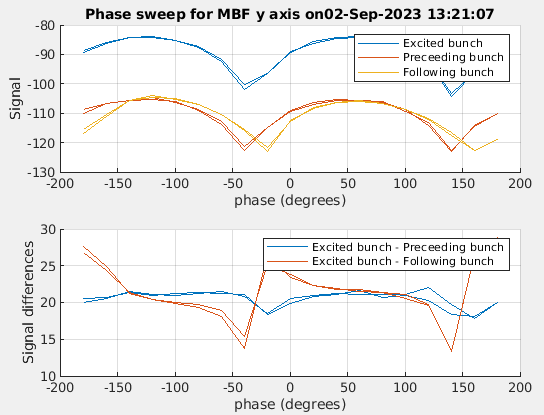
\includegraphics[width=\textwidth]{vlr_system_phase_scan_y.png}
        \caption{Vertical axis: Anywhere between $-30^\circ$ and $30^\circ$ looks to be a reasonable working point as you are near the maximum signal of the excited bunch and the selectivity for the preceding and following bunch's are trading off one another.}
        \label{fig:frontend_system_phase_scan_y}
    \end{subfigure}
    
    \begin{subfigure}[b]{0.45\textwidth}
        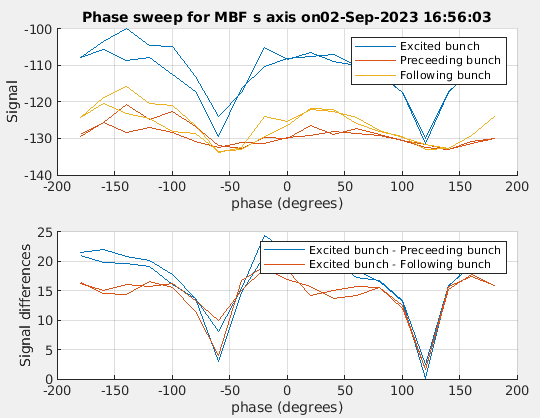
\includegraphics[width=\textwidth]{vlr_system_phase_scan_s.png}
        \caption{longitudinal axis: $-20^\circ$ looks to be a reasonable working point as it has the best selectivity while being close to the maximum signal to noise.}
        \label{fig:frontend_system_phase_scan_z}
    \end{subfigure}
    \caption{Example system phase results}
    \label{fig:frontend_system_phase_scan}
\end{figure}
\begin{tcolorbox}
\textbf{Note: }If the graphs are significantly asymmetric re-run the phase scan to check.

\textbf{Note:} If there are missing data points it can indicate that the DORIS system has unlocked. In this case you may need to inject a little more charge into the target bucket.
\end{tcolorbox}

\subsubsection{Clock phase scan} 
The following Matlab code will run a clock phase scan on each axis sequentially. The graphs will be displayed, and the data is automatically stored. 

\begin{minted}{matlab}
    >> BBBFE_clock_phase_scan('X', single_bunch_location)
    >> BBBFE_clock_phase_scan('Y', single_bunch_location)
    >> BBBFE_clock_phase_scan('S', single_bunch_location)
\end{minted}
Figure \ref{fig:frontend_clock_phase_scan} shows an example of the output. You use the same assessment as for the system phase scans.
\begin{tcolorbox}
\textbf{Note:} X and Y share a clock so you have to optimise both axes together.
\end{tcolorbox}

\begin{figure}[hbt]
   \centering
    \begin{subfigure}[b]{0.48\textwidth}
        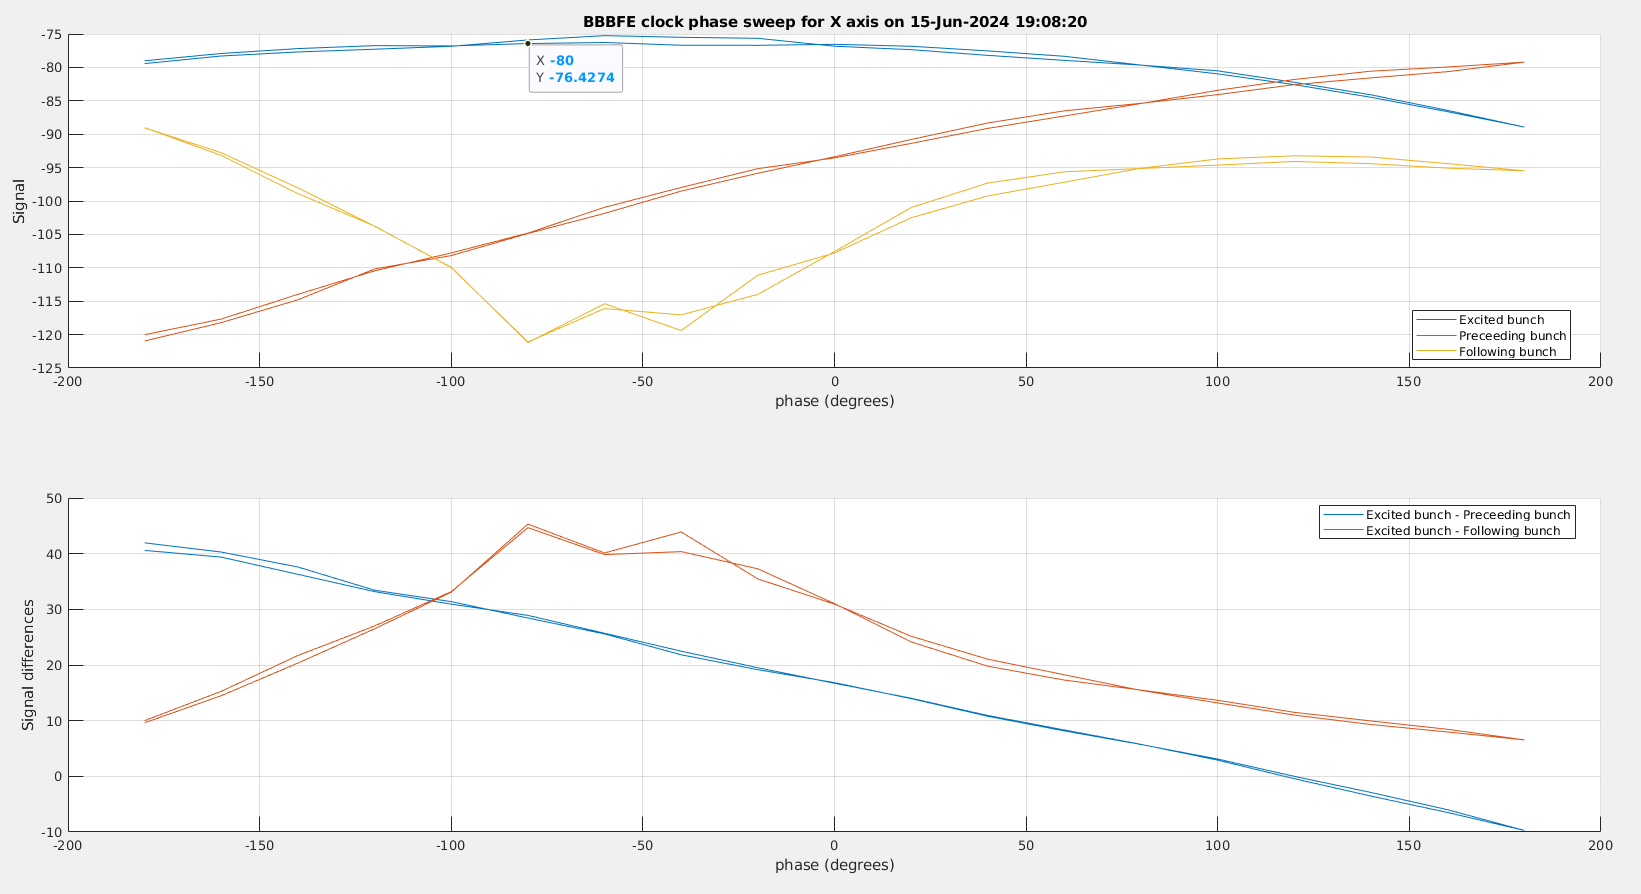
\includegraphics[width=\textwidth]{vlr_clock_phase_scan_x.png}
        \caption{Horizontal axis: $-80^\circ$ looks to be a reasonable working point.}
        \label{fig:frontend_clock_phase_scan_x}
    \end{subfigure}
    \begin{subfigure}[b]{0.48\textwidth}
        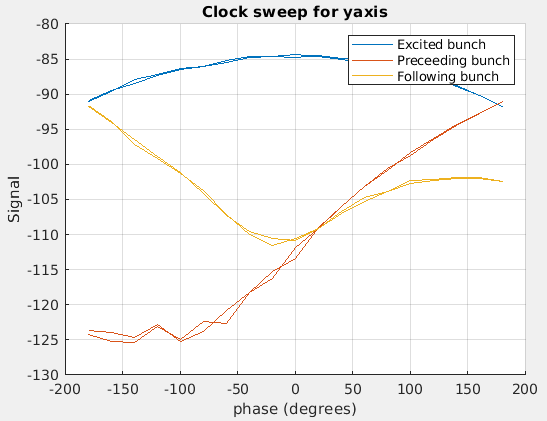
\includegraphics[width=\textwidth]{vlr_clock_phase_scan_y.png}
        \caption{Vertical axis: $-80^\circ$ looks to be a reasonable working point.}
        \label{fig:frontend_clock_phase_scan_y}
    \end{subfigure}
    
    \begin{subfigure}[b]{0.45\textwidth}
        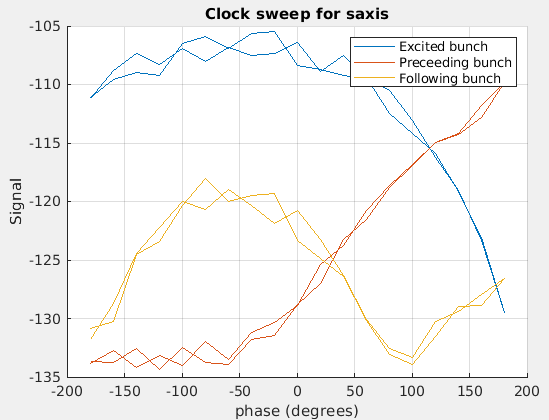
\includegraphics[width=\textwidth]{vlr_clock_phase_scan_s.png}
        \caption{longitudinal axis: $30^\circ$ looks to be a reasonable working point.}
        \label{fig:frontend_clock_phase_scan_z}
    \end{subfigure}
    \caption{Example clock phase results}
    \label{fig:frontend_clock_phase_scan}
\end{figure}

\begin{tcolorbox}
\textbf{Note:} Check the bunch standard deviation graphs to check that the motion is still only in a single bucket. If it is split over two then you may have to choose an alternative working phase.
\end{tcolorbox}

Once the system phase and clock phase are optimised then the tuning of the front end is complete.

The next step is to close the feedback loop.
\clearpage
\section{MBF closed loop setup}

\subsection{Machine settings}
\begin{itemize}
    \item {From an empty machine Inject to 30 - 50~mA into all bunches.}
    \begin{itemize}
    \item{this gives sufficient signal while staying below the instability threshold}
    \end{itemize}
    \item{Correct tune values to nominal.}
    \begin{itemize}
        \item{If you are struggling to get a reliable tune value try}
        \begin{itemize}
            \item{increasing the excitation -{\color{red}ADD SCREENSHOT} (Diagnostics $\rightarrow$ {\color{red}????})}
            \item{changing from fitted to maximum -{\color{red}ADD SCREENSHOT} (Diagnostics $\rightarrow$ {\color{red}????})}
        \end{itemize}
    \end{itemize}
    \item{Turn tune feedback off once tunes are nominal}
    \item{Correct orbit using fast orbit feedback (FOFB).}
\end{itemize}

\subsection{Initial measurement}
The following Matlab code will run a scan across all the harmonics of the tune on each axis sequentially. The graphs will be displayed, and the data is automatically stored.
\begin{minted}{matlab}
    >> modscan_all('x') 
    >> modscan_all('y') 
    >> modscan_all('s') 
\end{minted}
\clearpage
\subsection{Assessment} 

Use the modescan results to assess whether the closed loop delay is good enough.
 \begin{figure}[hbt]
   \centering
    \begin{subfigure}[b]{0.48\textwidth}
        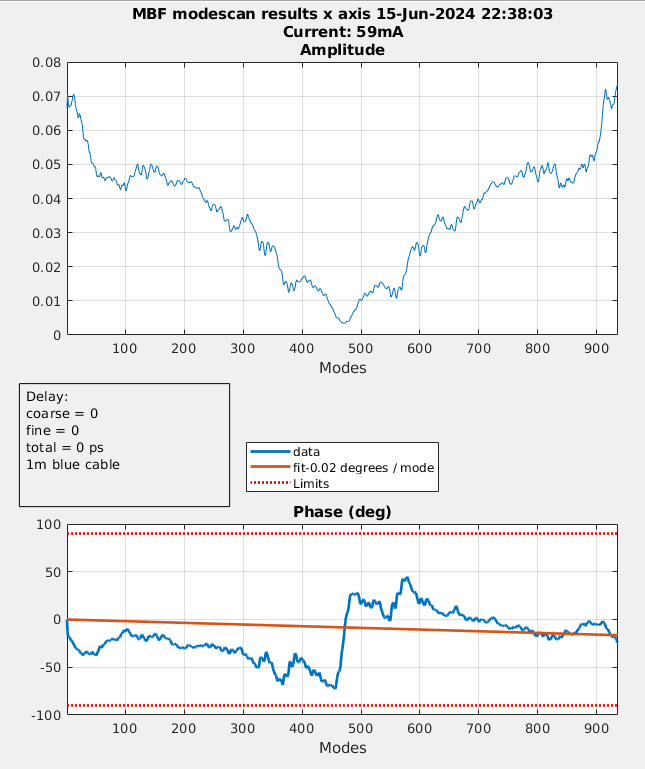
\includegraphics[width=\textwidth]{modescan_x.png}
        \caption{In this case the phase is ranging from $-70^\circ$ to $50^\circ$ and there is almost no residual gradient along the modes. Although any further increase in this range would be concerning and would warrant further investigation.}
        \label{fig:example_modescan_x}
    \end{subfigure}
    \begin{subfigure}[b]{0.48\textwidth}
        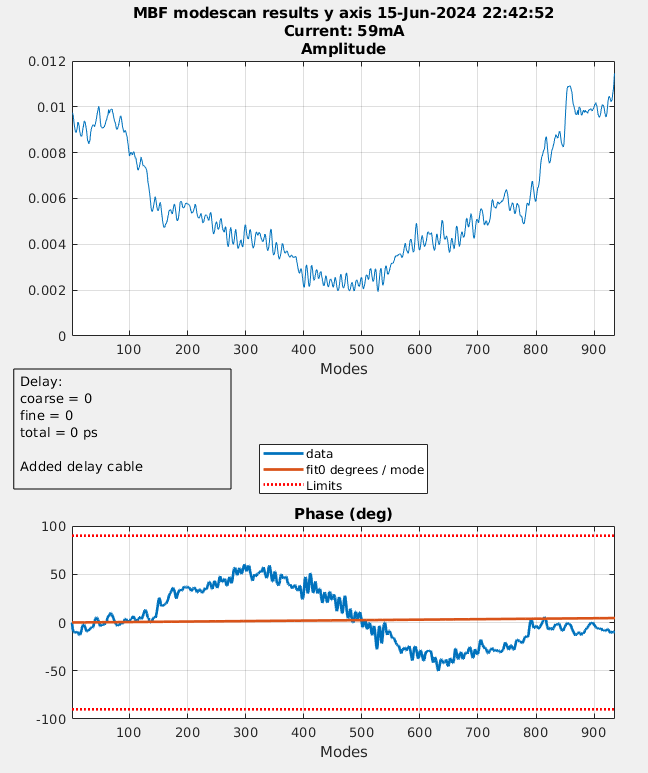
\includegraphics[width=\textwidth]{modescan_y.png}
        \caption{The phase is ranging from $-50^\circ$ to $50^\circ$ and there is almost no residual gradient along the modes indicating that the loop delay is close to the required value.}
        \label{fig:example_modescan_y}
    \end{subfigure}
\end{figure}

 
The amplitude should be fairly symmetric in the modes axis. If there is a significant change in the lowest modes only then check you have filled all bunches. The fewer bunches you fill the larger the distortion of the lower mode response becomes. 

The phase variation should be much less that $\pm90^\circ$ and the extents should be balanced between going above and below zero.

By taking a linear fit along the modes one can estimate the required electrical delay needing to be added or removed from the loop. Positive gradient means length must be added while negative gradient means length must be removed.

This error in the electrical length / delay / phase can be fixed in the following ways. 

First see if a DAC delay can fix it (using the control panel shown in figure \ref{fig:DAC_delay_screen}). This is only available in 2ns steps.

Otherwise, we must change cable lengths. The easiest place to do this is at the output port of the output amplifier. As shown in figure \ref{fig:output_amplifiers}
\clearpage
\subsection{Tuning the loop delay} 

Rerun the modescan code after each change.

The aim of this exercise is to get the extents of the phase trace comfortably fit within the $\pm90^\circ$ limits (similar to the result show in figure \ref{fig:example_modescan_y}). 

\begin{tcolorbox}
\textbf{Note:} The spec for the phase variation of the output amplifier alone is $\pm~20$.
\end{tcolorbox}

\subsubsection{Tuning the DAC delay} 
This allows additional phase (delay) to be added to the closed loop.
\begin{figure}[ht]
    \centering
    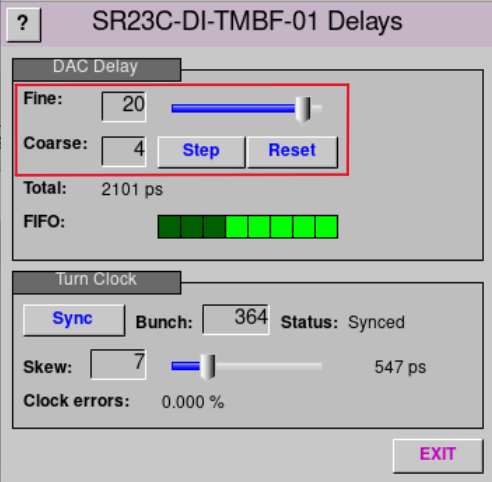
\includegraphics[width=0.5\linewidth]{DAC_delay.png}
    \caption{DAC delay control screen}
    \label{fig:DAC_delay_screen}
\end{figure}
\begin{tcolorbox}
\textbf{Note:} The DAC delay is shared between X and Y axes so it may be required to retune both.
\end{tcolorbox}

Use this setting first to get as close as possible to the target performance. Any remaining adjustment will have to be done with physical cable length changes. 
\clearpage
\subsubsection{Tuning the cable length} 
Modify the cable length until the extents of the phase trace comfortably fit within the limits.  
\begin{figure}[ht]
    \centering
    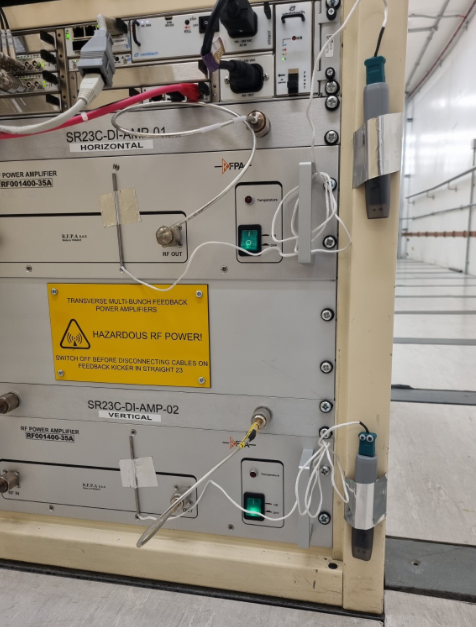
\includegraphics[width=0.6\linewidth]{amp_front.png}
    \caption{Output amplifiers showing the RF cables to adjust}
    \label{fig:output_amplifiers}
\end{figure}
A large phase variation even when the overall gradient is close to zero indicates that a component is failing – probably the output amplifier. So, a hardware change and a retuning of the frontend is required. (see documentation on tuning up the frontend)
\subsubsection{Tuning the FIR phase}
The overall phase of the feedback loop should be 180 degrees. So the last step is to change the FIR phase setting so the readback value is close to ($\pm~20$) 180.

At this point the full loop delay should be optimised
\clearpage

\section{MBF standard operational measurements}
\subsection{Machine setup} 
\begin{itemize}
    \item {Inject to 30mA 900 bunches (below the instability threshold)}
\end{itemize}

\subsection{Code to run}

The following Matlab code will run modescan, growdamp and spectra measurements for each axis sequentially. The data is stored automatically 
\begin{verbatim}
    >> mbf_startup_tests 
\end{verbatim}
\vspace{2mm}
The following explains how to run each separate standard measurement. However there are some common optional inputs.
\begin{minted}{matlab}
'plotting', 'yes' or 'no'. 
\end{minted}
Determines if the plotting is displayed. The raw data is saved in either case.
\begin{minted}{matlab}
'auto_setup', 'yes' or 'no'. 
\end{minted}
This determines whether to use the main scripts to reset the system to a known state. However this is dangerous if the machine is not in an intrinsically stable condition.
\begin{minted}{matlab}
'tunes', previously measured tune value.
\end{minted}
The default is to measure the tune as part of the measurement.
\subsubsection{Growdamp}
The top level code to run a growdamp measurement for each axis is; 
\begin{minted}{matlab}
    >> [~] = growdamp_all('x') 
    >> [~] = growdamp_all('y') 
    >> [~] = growdamp_all('s') 
\end{minted}

The parameters for the length of excitation and  capture are set in \verb|mbf_growdamp_config.m|.
 The \verb|mbf_growdamp_setup| code sets up the hardware for the correct type of measurement. 
 
 \verb|mbf_growdamp_capture| triggers the measurement, captures the data and stores it in the file structure defined in \verb|mbf_system_config|. 
\subsubsection{Modescan}
The top level code to run a modescan measurement for each axis is; 
\begin{minted}{matlab}
    >> modescan_all('x') 
    >> modescan_all('y') 
    >> modescan_all('s') 
\end{minted}

The \verb|mbf_modescan_setup| code sets up the hardware for the correct type of measurement. \verb|mbf_modescan_capture| triggers the measurement, captures the data and stores it in the file structure defined in \verb|mbf_system_config|. 
\subsubsection{Spectra}
The top level code to run a modescan measurement for each axis is; 
\begin{minted}{matlab}
    >> mbf_spectrum_all('x') 
    >> mbf_spectrum_all('y') 
    >> mbf_spectrum_all('s') 
\end{minted}

The \verb|mbf_spectrum_setup| code sets up the hardware for the correct type of measurement. \verb|mbf_spectrum_capture| triggers the measurement, captures the data and stores it in the file structure defined in \verb|mbf_system_config|. 

\section{MBF developmental measurements}
The MBF system is also used as an instrument for investigating the accelerator behaviour and the behaviour of the beam under different conditions. It can also be used as a driver for certain beam behaviours. These codes tend to be less well tested as they are often only used for particular investigations.
\subsection{Transverse damping}
\subsection{Emittance control}
\subsection{Bunch motion}
 \verb|mbf_bunch_motion_setup| sets up all three systems to use the appropriate triggers. 
 
 \verb|mbf_bunch_motion_capture| arms the systems, and once triggered by an external trigger, will capture and store the data.

\chapter{MBF Archival retrieval}

\section{Introduction}

All the MBF codes store their data in a common location with programmatically constructed names. Therefore, it is possible to extract and compare this data. 

\section{Getting the latest data} 

The simplest thing is to look at the last results taken. To do this simply run the command below on the Matlab command line. 
\begin{minted}{matlab}
   >> visualise_latest_mbf_results 
\end{minted}
 This will return analysed results for all the standard measurements.
 You can also get the code to save pngs of the graphs at a location of your choosing using optional flags.
\begin{minted}{matlab}
>> visualise_latest_mbf_results('save_graphs', 'yes', 'out_path', [your desired location])
\end{minted}
It is possible to change the x axis of the Growdamp measurement by using the  \verb+growdamp_plot_mode+ optional input.
\begin{minted}{matlab}
    >> visualise_latest_mbf_results('growdamp_plot_mode', 'freq') 
\end{minted}
Will put the output on a frequency scale rather than the usual mode scale 
\begin{minted}{matlab}
    >> visualise_latest_mbf_results('growdamp_plot_mode', 'pos') 
\end{minted}
Will reorganise the modes to be numbered 0:935 rather than –468:468 

Figure \ref{fig:growdamp_example} is an example of the output for Growdamp, figure \ref{fig:modescan_example} of Modescan measurements and figure \ref{fig:spectrum_example} of spectral measurements.

 \begin{figure}[hbt]
   \centering
    \begin{subfigure}[b]{0.45\textwidth}
        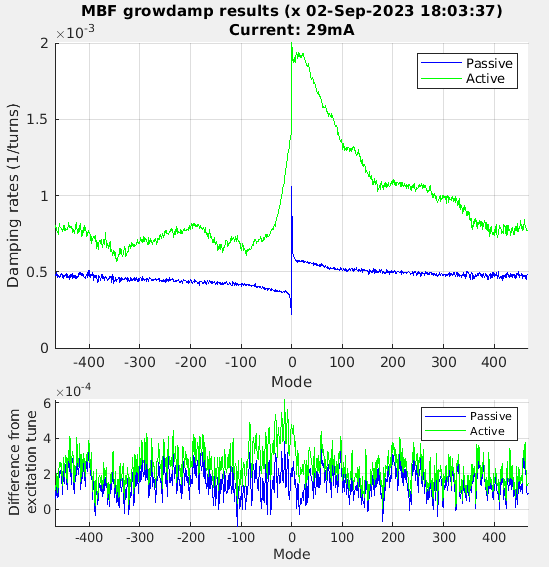
\includegraphics[width=\textwidth]{vlr_growdamp_x.png}
        \caption{Horizontal axis}
        \label{fig:growdamp_example_x}
    \end{subfigure}
    \begin{subfigure}[b]{0.45\textwidth}
        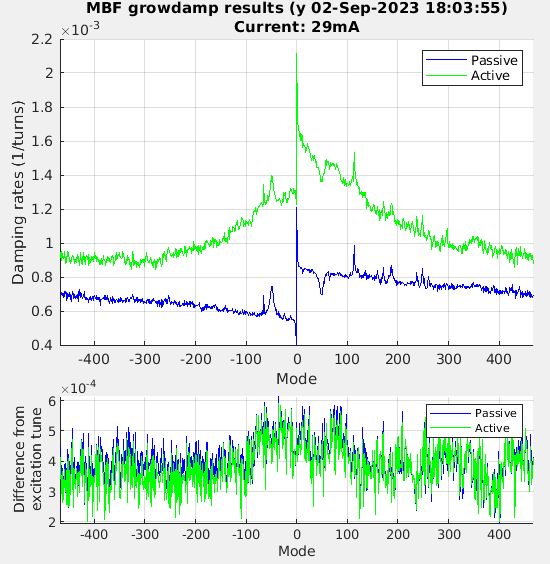
\includegraphics[width=\textwidth]{vlr_growdamp_y.png}
        \caption{Vertical axis}
        \label{fig:growdamp_example_y}
    \end{subfigure}
    
    \begin{subfigure}[b]{0.45\textwidth}
        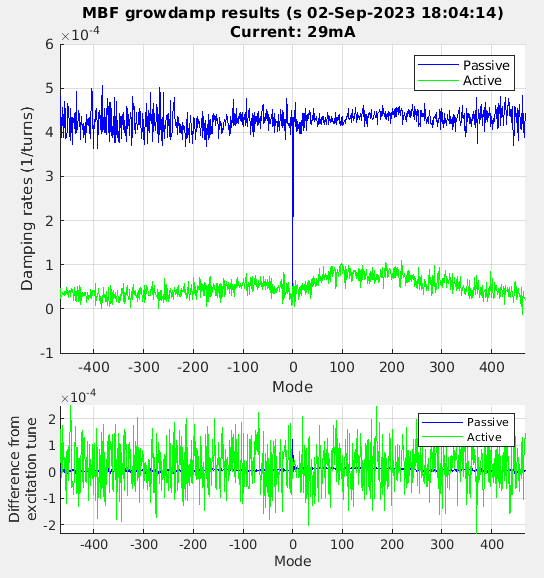
\includegraphics[width=\textwidth]{vlr_growdamp_s.png}
        \caption{longitudinal axis}
        \label{fig:growdamp_example_z}
    \end{subfigure}
    \caption{Example Growdamp results}
    \label{fig:growdamp_example}
\end{figure}

 \begin{figure}[hbt]
   \centering
    \begin{subfigure}[b]{0.45\textwidth}
        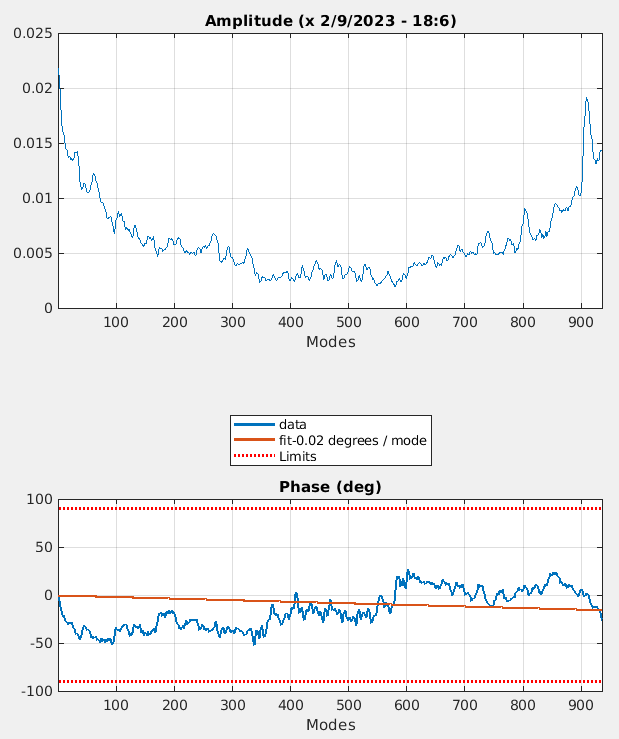
\includegraphics[width=\textwidth]{vlr_modescan_x.png}
        \caption{Horizontal axis}
        \label{fig:modescan_example_x}
    \end{subfigure}
    \begin{subfigure}[b]{0.45\textwidth}
        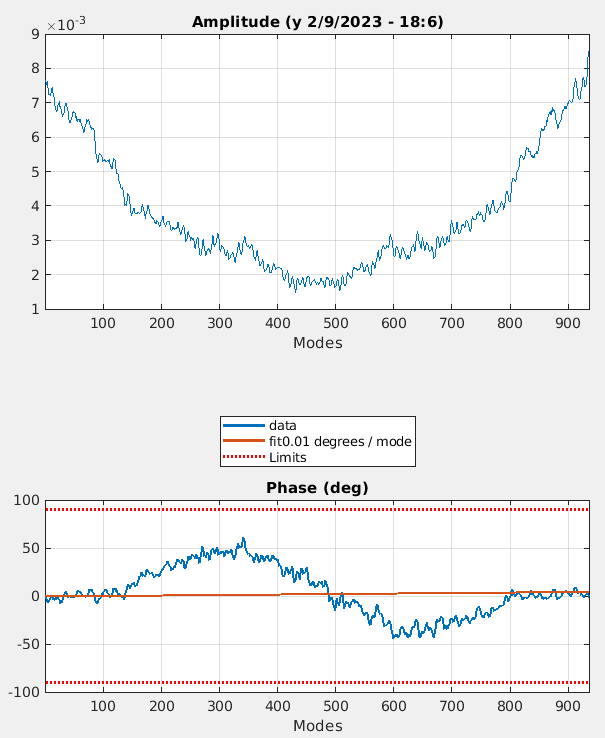
\includegraphics[width=\textwidth]{vlr_modescan_y.png}
        \caption{Vertical axis}
        \label{fig:modescan_example_y}
    \end{subfigure}
    
    \begin{subfigure}[b]{0.45\textwidth}
        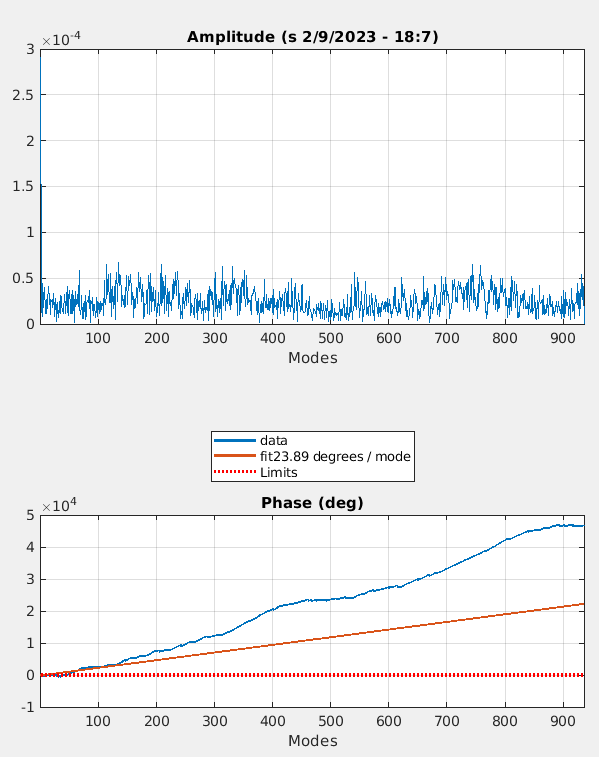
\includegraphics[width=\textwidth]{vlr_modescan_s.png}
        \caption{longitudinal axis}
        \label{fig:modescan_example_z}
    \end{subfigure}
    \caption{Example modescan results}
    \label{fig:modescan_example}
\end{figure}

 The spectra graphs show the residual motion after all feedbacks have been applied.

 \begin{figure}[hbt]
   \centering
    \begin{subfigure}[b]{0.45\textwidth}
        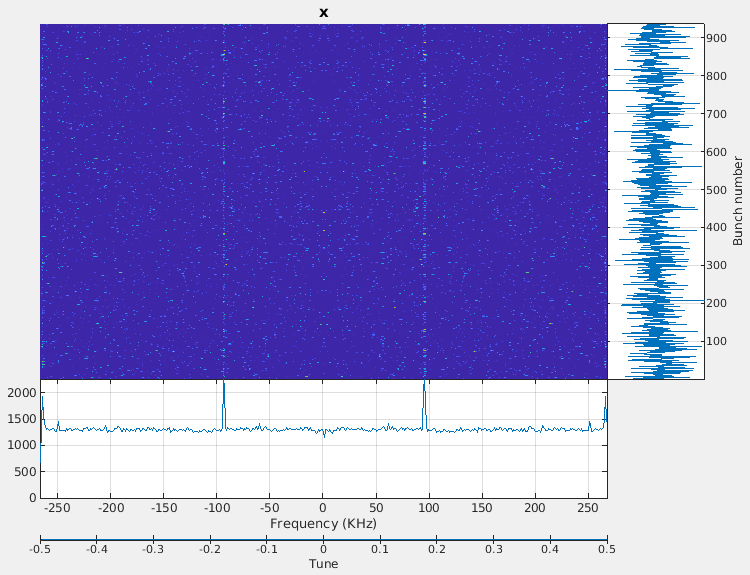
\includegraphics[width=\textwidth]{vlr_spectrum_x.png}
        \caption{Horizontal axis}
        \label{fig:spectrum_example_x}
    \end{subfigure}
    \begin{subfigure}[b]{0.45\textwidth}
        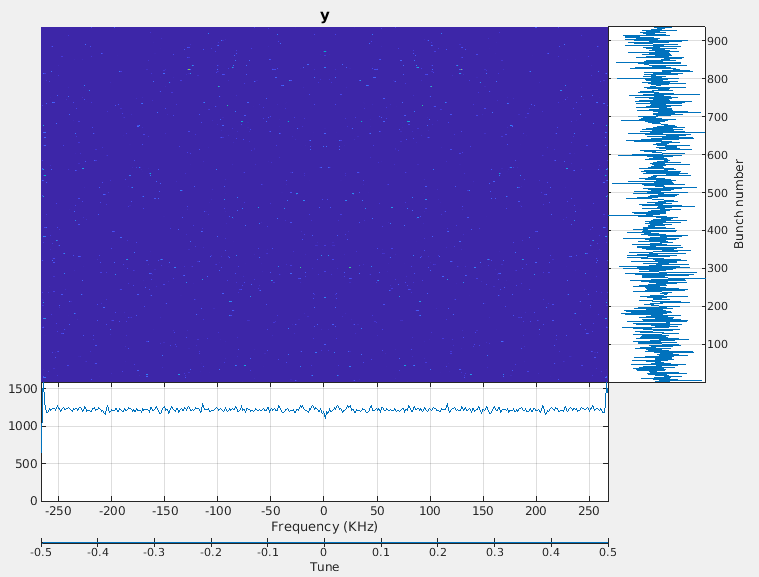
\includegraphics[width=\textwidth]{vlr_spectrum_y.png}
        \caption{Vertical axis}
        \label{fig:spectrum_example_y}
    \end{subfigure}
    
    \begin{subfigure}[b]{0.45\textwidth}
        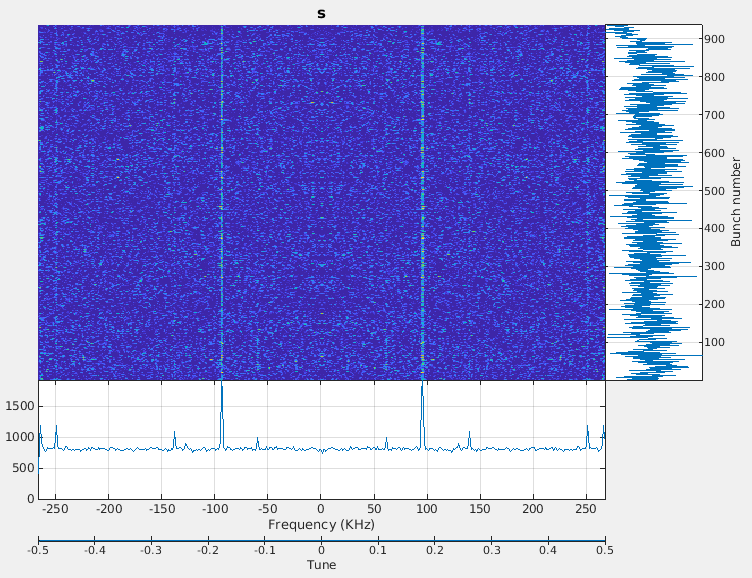
\includegraphics[width=\textwidth]{vlr_spectrum_s.png}
        \caption{longitudinal axis}
        \label{fig:spectrum_example_z}
    \end{subfigure}
    \caption{Example spectrum results- PLACEHOLDER}
    \label{fig:spectrum_example}
\end{figure}
\clearpage
\section{Frontend tuning results}
By running \verb|visualise_latest_bbbfe_results| it will output the results from the latest results from the DORIS and frontend tuning.
\begin{minted}{matlab}
>> visualise_latest_BBFE_results
\end{minted}
You can also get the code to save pngs of the graphs at a location of your choosing using optional flags.
\begin{minted}{matlab}
>> visualise_latest_BBFE_results('save_graphs', 'yes', 'out_path', [your desired location])
\end{minted}
\begin{figure}[hbt]
   \centering
    \begin{subfigure}[b]{0.45\textwidth}
        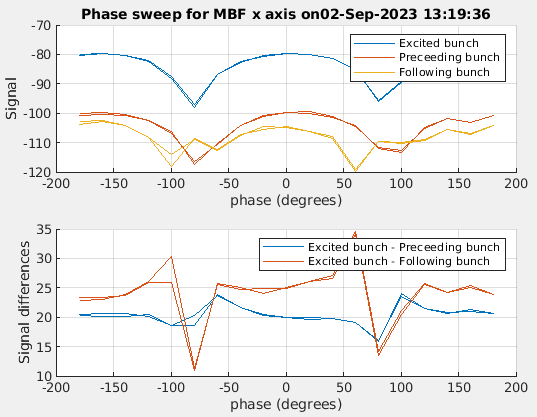
\includegraphics[width=\textwidth]{vlr_system_phase_scan_x.png}
        \caption{Horizontal axis}
        \label{fig:system_phase_example_x}
    \end{subfigure}
    \begin{subfigure}[b]{0.45\textwidth}
        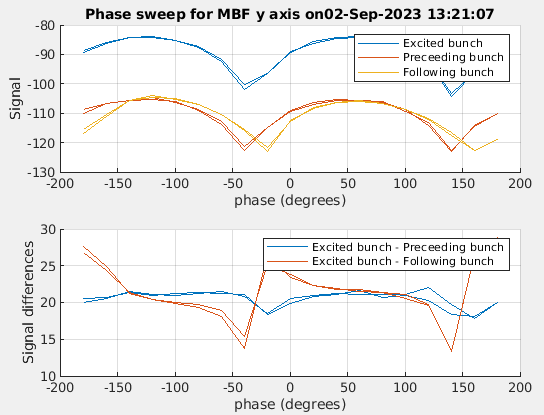
\includegraphics[width=\textwidth]{vlr_system_phase_scan_y.png}
        \caption{Vertical axis}
        \label{fig:system_phase_example_y}
    \end{subfigure}
    
    \begin{subfigure}[b]{0.45\textwidth}
        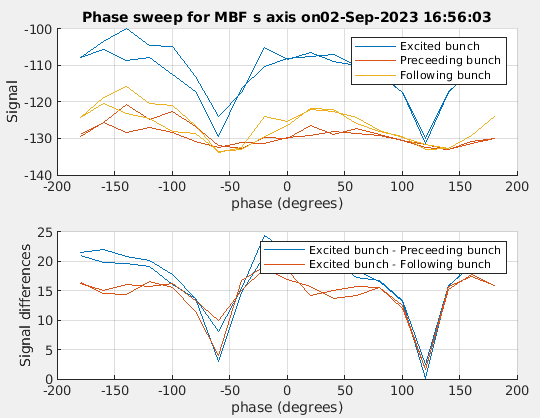
\includegraphics[width=\textwidth]{vlr_system_phase_scan_s.png}
        \caption{longitudinal axis}
        \label{fig:system_phase_example_z}
    \end{subfigure}
    \caption{Example system phase results}
    \label{fig:system_phase_example}
\end{figure}

\begin{figure}[hbt]
   \centering
    \begin{subfigure}[b]{0.45\textwidth}
        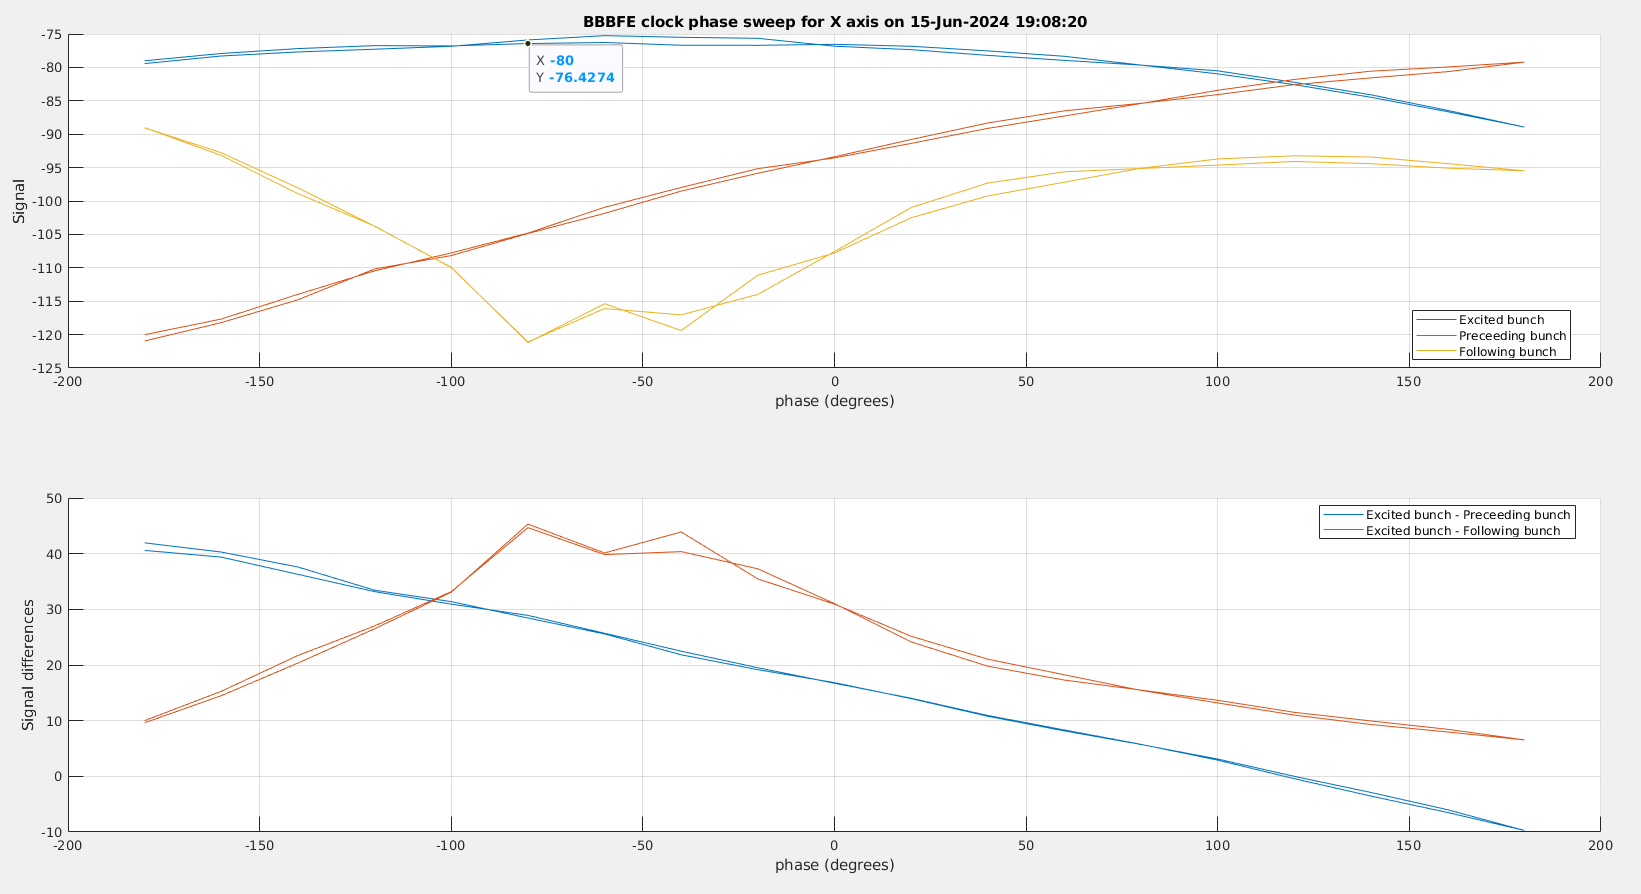
\includegraphics[width=\textwidth]{vlr_clock_phase_scan_x.png}
        \caption{Horizontal axis}
        \label{fig:clock_phase_example_x}
    \end{subfigure}
    \begin{subfigure}[b]{0.45\textwidth}
        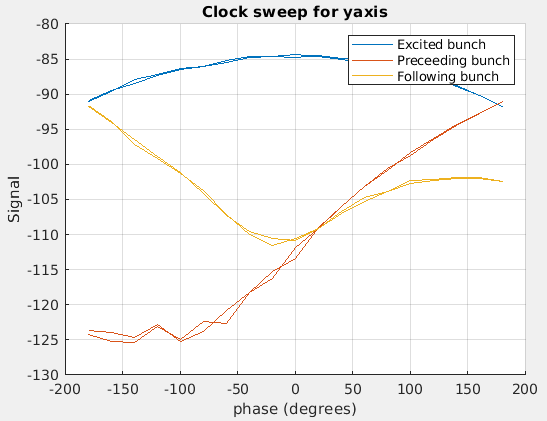
\includegraphics[width=\textwidth]{vlr_clock_phase_scan_y.png}
        \caption{Vertical axis}
        \label{fig:clock_phase_example_y}
    \end{subfigure}
    
    \begin{subfigure}[b]{0.45\textwidth}
        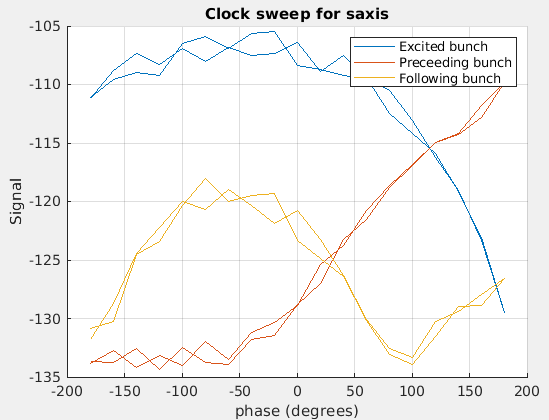
\includegraphics[width=\textwidth]{vlr_clock_phase_scan_s.png}
        \caption{longitudinal axis}
        \label{fig:clock_phase_example_z}
    \end{subfigure}
    \caption{Example clock phase results}
    \label{fig:clock_phase_example}
\end{figure}

\clearpage
\section{Getting any historic data} 

A more flexible way is to set up the time period you are interested in looking at and use the measurement specific retrieval tool. 

You can set up the period of interest by using a modified version the following example code. 
\begin{minted}{matlab}
    >> start_datenum = datetime('16/04/2023_21:38',...
        'InputFormat','dd/MM/yyyy_HH:mm'); 
    >> end_datenum = datetime('16/06/2023_22:55',...
        'InputFormat','dd/MM/yyyy_HH:mm'); 
    >> date_range = [start_datenum, end_datenum]; 
\end{minted}
Starting with growdamp data, the following command will extract any measurements taken within the date range for the y axis and then plot them on top of one another. An example of this is shown in figure \ref{fig:growdamp_collate}.
\begin{minted}{matlab}
    >> conditioned_data = mbf_growdamp_archival_retrieval('y',...
        date_range); 
\end{minted}
\begin{figure}[ht]
    \centering
    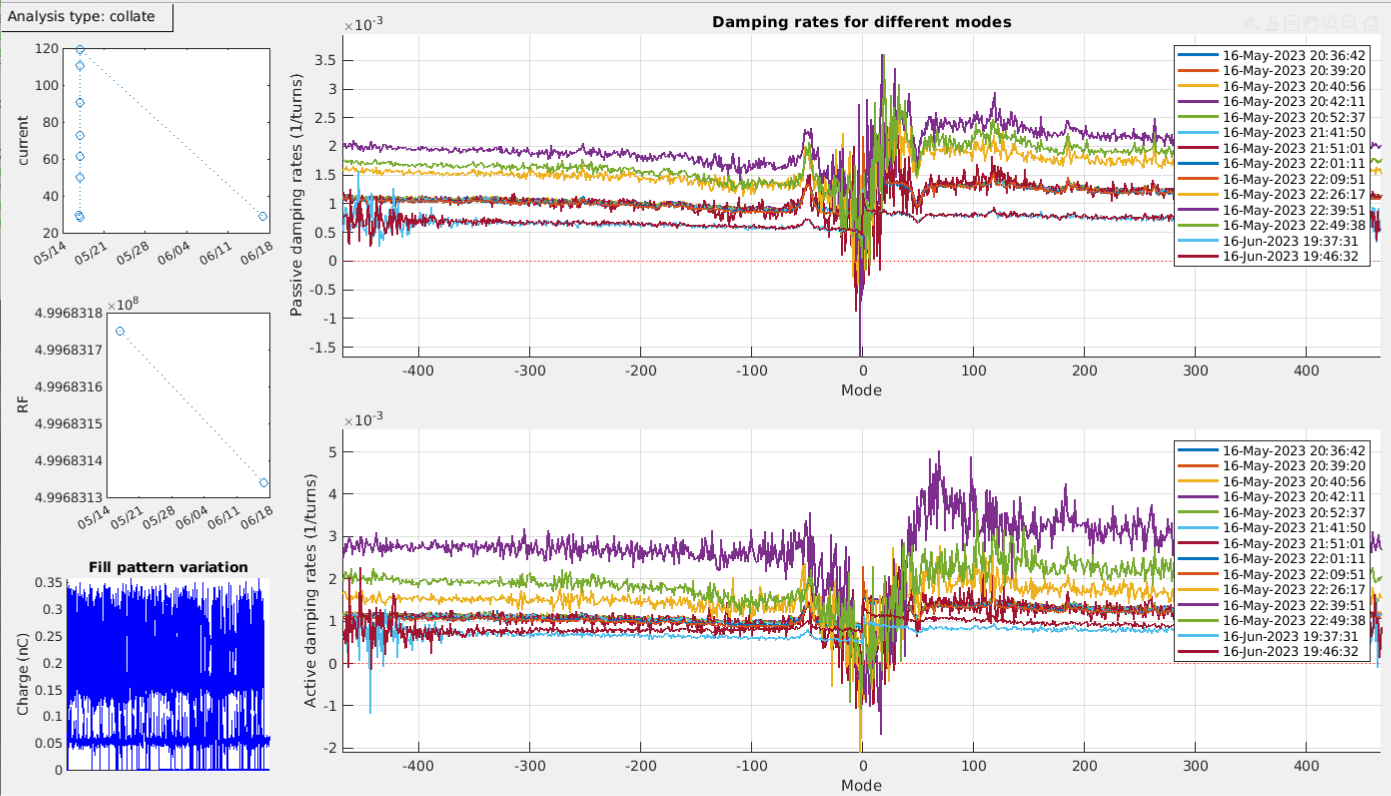
\includegraphics[width=1\linewidth]{growdamp_collate.png}
    \caption{Collated growdamp results}
    \label{fig:growdamp_collate}
\end{figure}

This allows easy identification of changes in behaviour 


As machine conditions can be different it is possible to filter on current range and RF frequency range 

For example, by setting the \verb+current_range+ optional input we can select only measurements which were taken between 2mA and 40mA (figure \ref{fig:growdamp_collated_limit_current_range}).

\begin{minted}{matlab}
    >> conditioned_data = mbf_growdamp_archival_retrieval('y',...
        date_range, 'current_range', [2 40]); 
\end{minted}

This is often useful to ensure that any measurements used are below instability thresholds. 
\begin{figure}[ht]
    \centering
    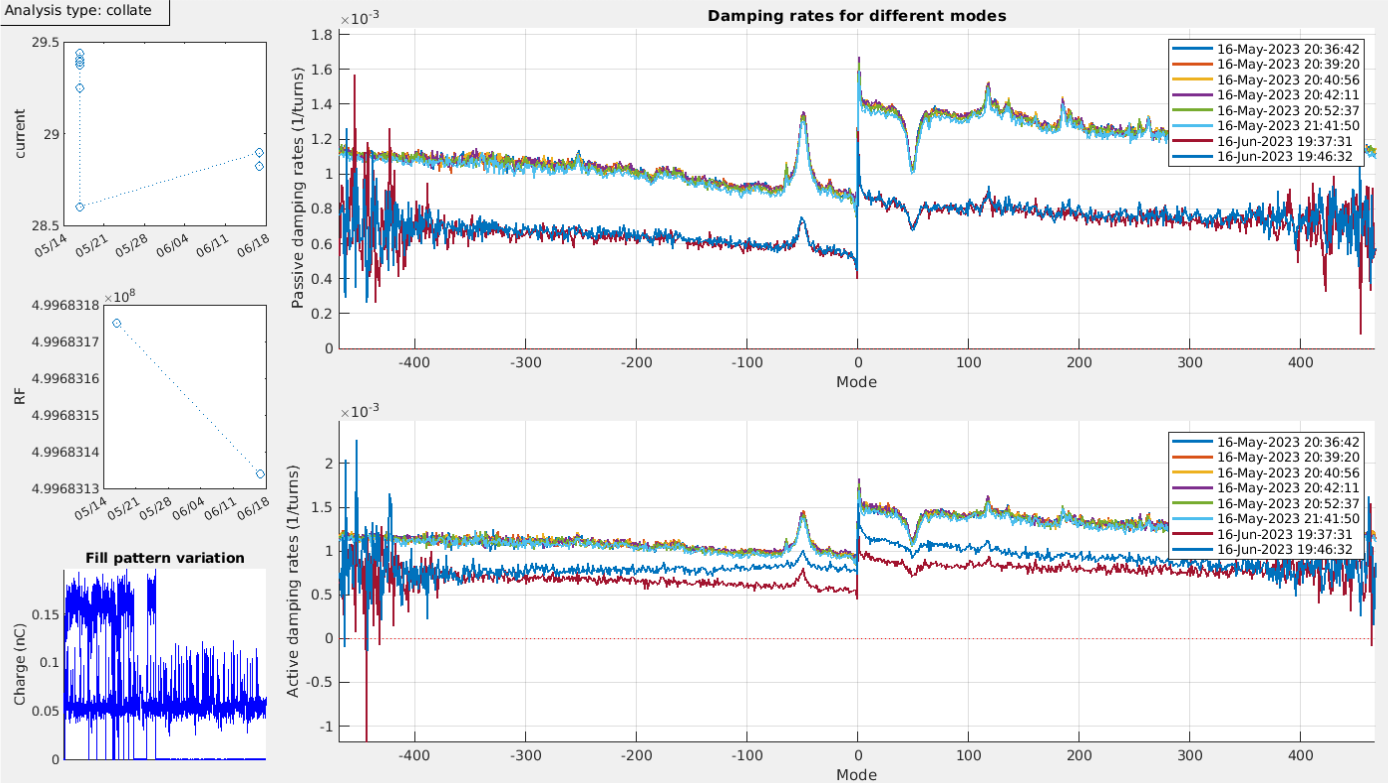
\includegraphics[width=1\linewidth]{growdamp_collate_limit_current_range.png}
    \caption{Collated growdamp results only returning results which are within the specified current range.}
    \label{fig:growdamp_collated_limit_current_range}
\end{figure}
One common set of measurements beyond simple comparisons is plotting the measurements against a changing machine parameter (usually current) 

Although it is possible to extract such relationships from the data just using the variation over time, it is more usual to have a dedicated measurement set for the purpose. In this case you would set the period to only contain data from that experiment. Then you would run the retrieval with the analysis type set to sweep and then set the appropriate parameter to sweep over (again it is usually current but any variable in the datasets can be used). Figure \ref{fig:growdamp_parameter_sweep} shows an example of this.
\begin{minted}{matlab}
    >> conditioned_data = mbf_growdamp_archival_retrieval('y', ...
        date_range, 'analysis_type', 'sweep',...
        'sweep_parameter', 'current'); 
\end{minted}
\begin{figure}[ht]
    \centering
    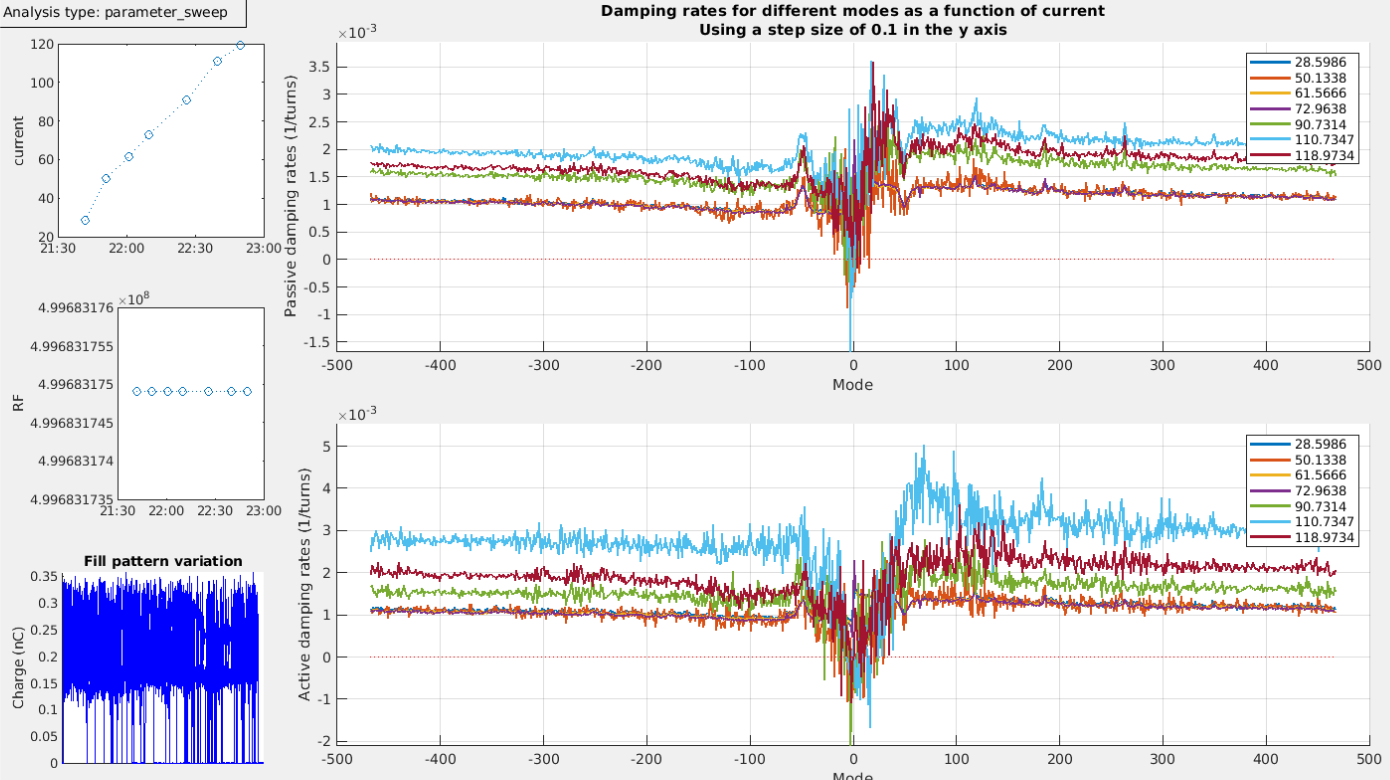
\includegraphics[width=1\linewidth]{growdamp_parameter_sweep.png}
    \caption{Growdamp results against a swept parameter. In this case the beam current. Note: These are placeholder graphs.}
    \label{fig:growdamp_parameter_sweep}
\end{figure}
At this point further analysis is possible. In the case of a current sweep, it is possible to predict the current which individual modes will go unstable. (figure \ref{fig:growdamp_parameter_sweep_further_analysis}). 
\begin{figure}[ht]
    \centering
    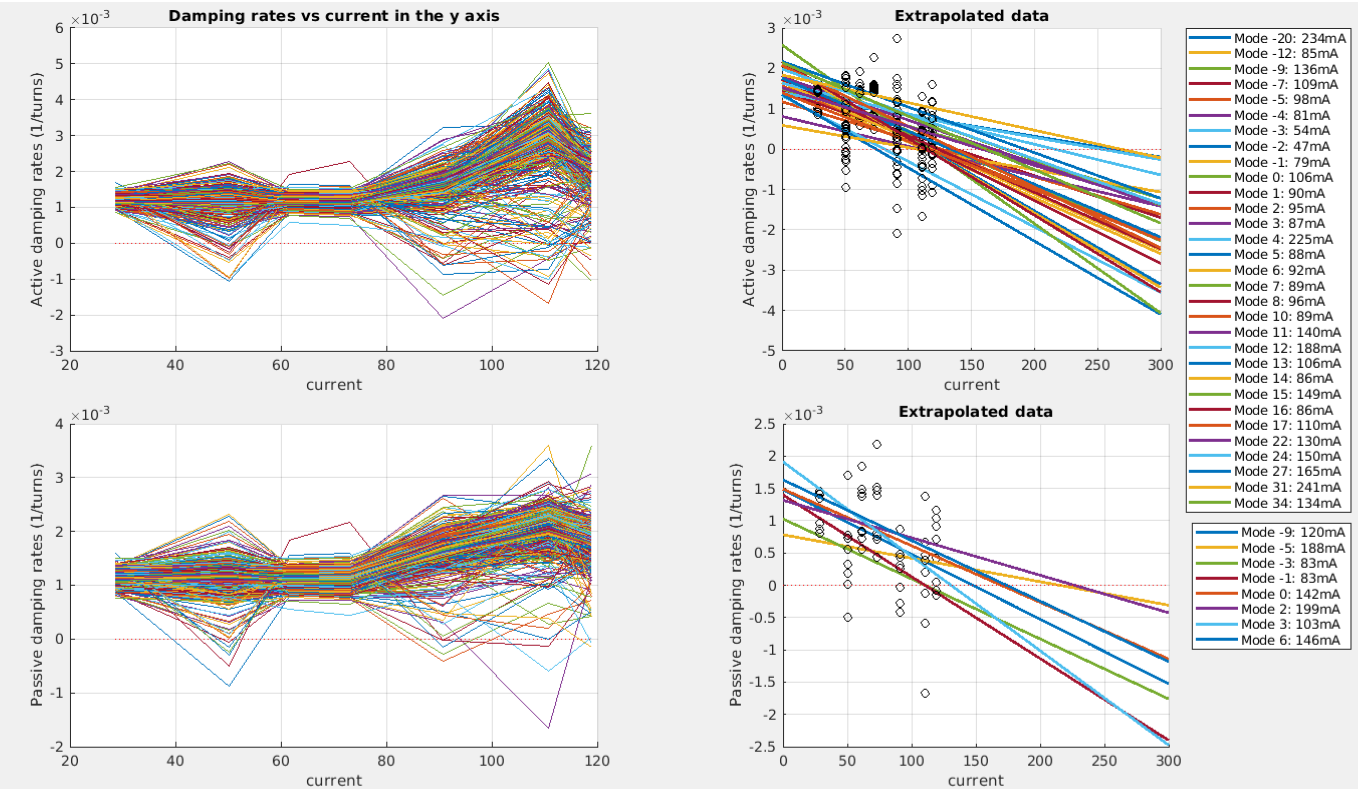
\includegraphics[width=1\linewidth]{growdamp_parameter_sweep_further_analysis.png}
    \caption{Results from further analysis of the current dependent growdamp data. Note: These are placeholder graphs.}
    \label{fig:growdamp_parameter_sweep_further_analysis}
\end{figure}
\clearpage
Modescan data retrieval is much the same as the growdamp retrieval. Once the date range is set up the following code will extract and display all results from the y axis (figure \ref{fig:modescan_collate}).  
\begin{minted}{matlab}
    >> conditioned_data = mbf_modescan_archival_retrieval('y',...
        date_range); 
\end{minted}
 \begin{figure}[ht]
     \centering
     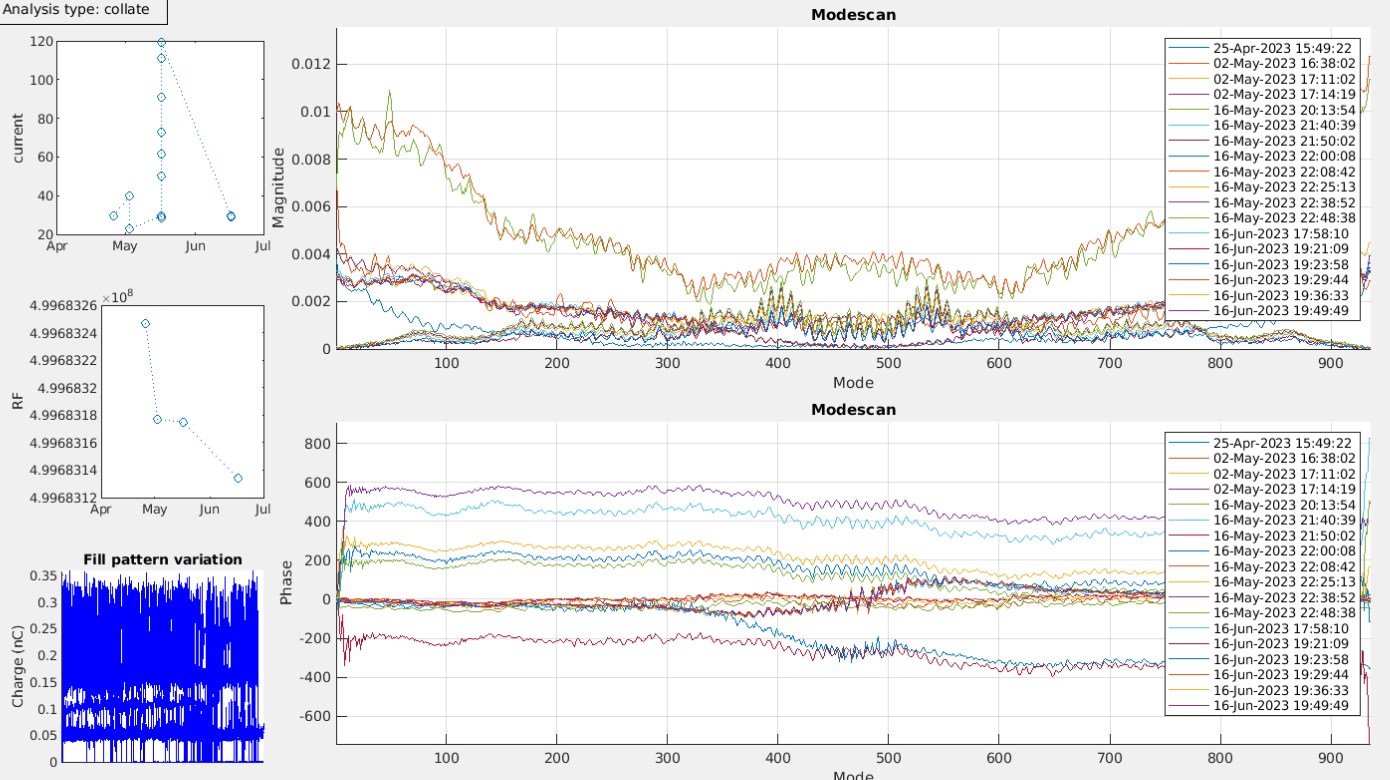
\includegraphics[width=1\linewidth]{modescan_collate.png}
     \caption{Collated modescan results}
     \label{fig:modescan_collate}
 \end{figure}

As before you can filter on current range(figure \ref{fig:modescan_collate_limited_range}).  
\begin{minted}{matlab}
    >> conditioned_data = mbf_modescan_archival_retrieval('y',...
        date_range, 'current_range', [2 40]); 
\end{minted}
 \begin{figure}[ht]
     \centering
     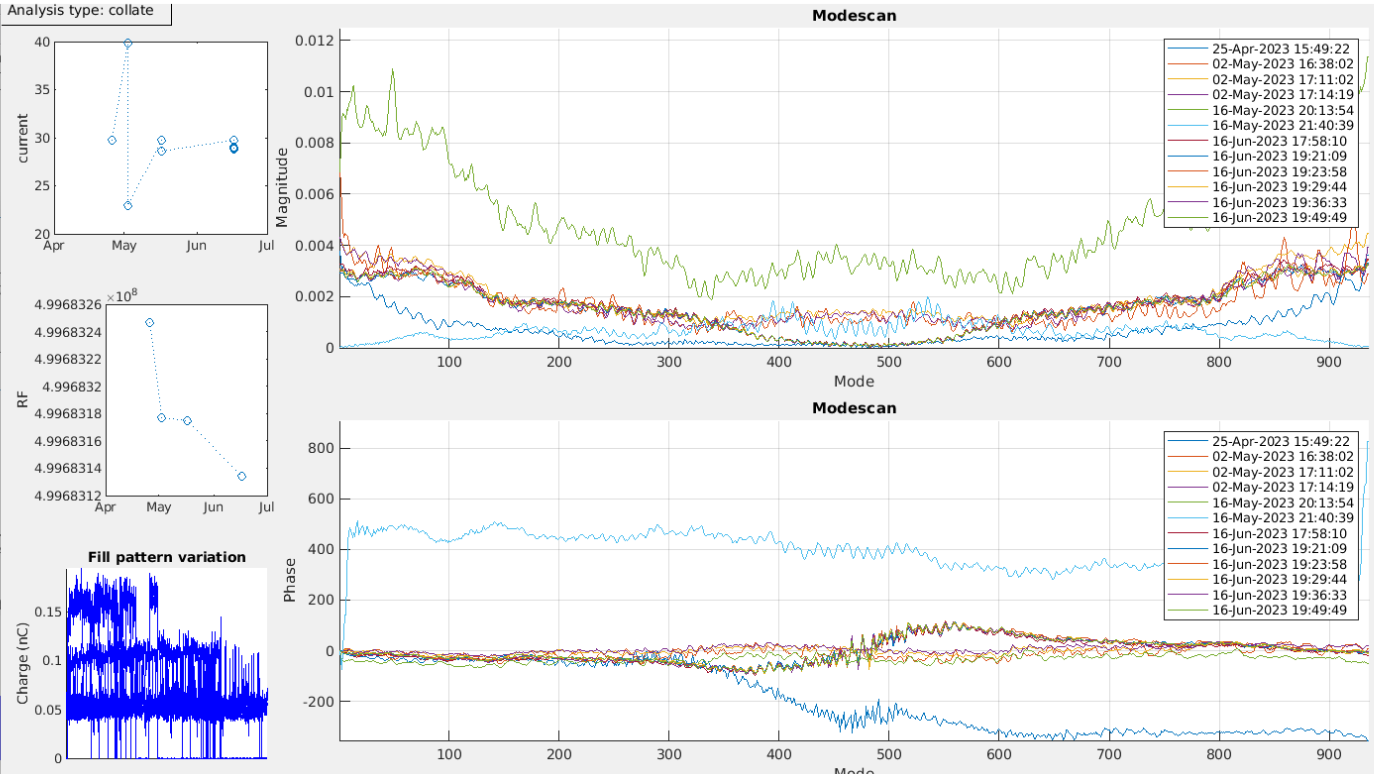
\includegraphics[width=1\linewidth]{modescan_collate_limited_range.png}
     \caption{Collated modescan results restricted to the specified current range.}
     \label{fig:modescan_collate_limited_range}
 \end{figure}

And can plot against a parameter sweep  (figure \ref{fig:modescan_parameter_sweep}). 
\begin{minted}{matlab}
    >> conditioned_data = mbf_modescan_archival_retrieval('y',...
        date_range, 'analysis_type', 'sweep',...
        'sweep_parameter', 'current'); 
\end{minted}
 \begin{figure}[ht]
     \centering
     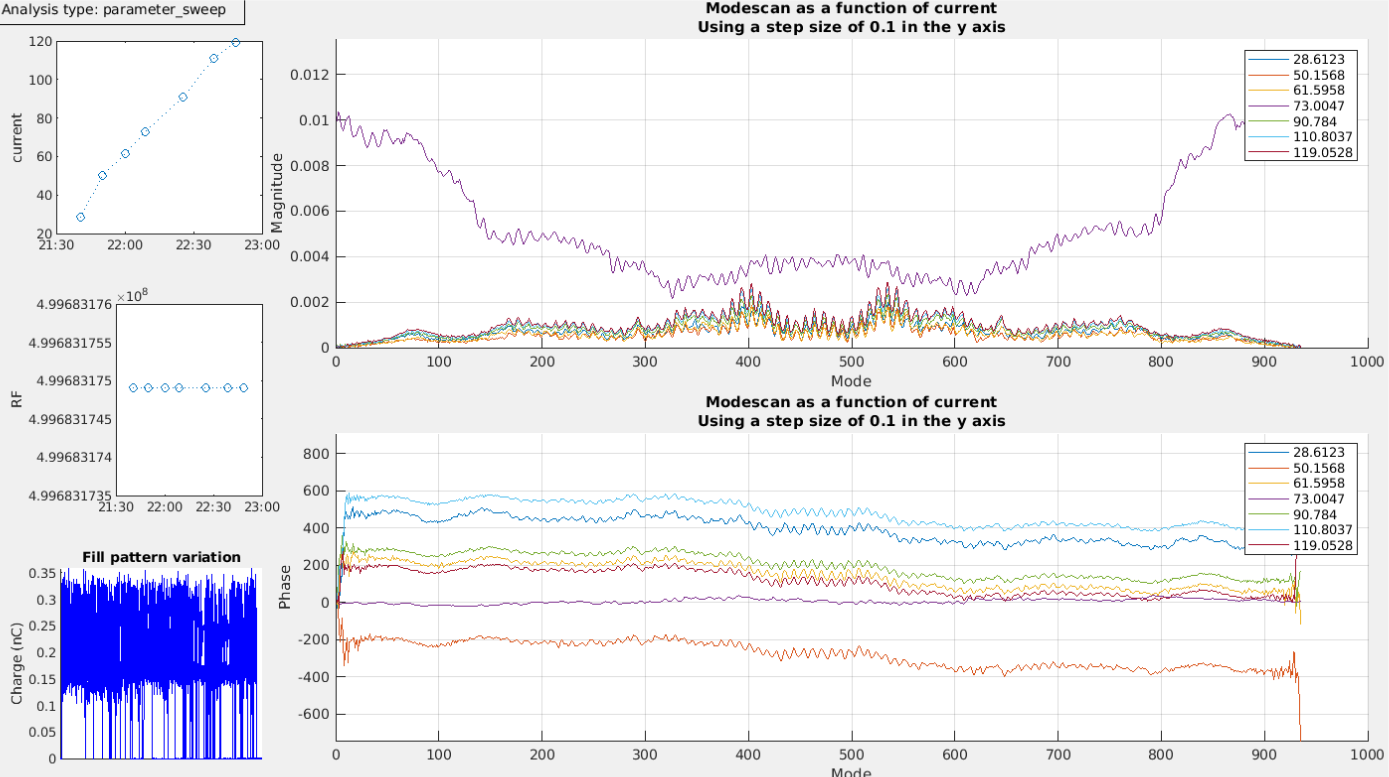
\includegraphics[width=1\linewidth]{modescan_parameter_sweep.png}
     \caption{Growdamp results against a swept parameter. In this case the beam current.}
     \label{fig:modescan_parameter_sweep}
 \end{figure}
\clearpage
Spectra 

Tune sweep over modes 
\clearpage

\end{document}




